% this TeX file provides an awesome example of how TeX will make super 
% awesome tables, at the cost of your of what happens when you try to make a
% table that is very complicated.
% Originally turned in for Dr. Nico's Security Class
\documentclass[11pt]{article}
\usepackage{floatrow}
\usepackage{url}
% Use wide margins, but not quite so wide as fullpage.sty
\marginparwidth 0.5in 
\oddsidemargin 0.25in 
\evensidemargin 0.25in 
\marginparsep 0.25in
\topmargin 0.25in 
\textwidth 6in \textheight 8 in
% That's about enough definitions

% multirow allows you to combine rows in columns
\usepackage{multirow}
% tabularx allows manual tweaking of column width
\usepackage{tabularx,graphicx,amssymb,gensymb,amsmath,mathtools}
% longtable does better format for tables that span pages
\usepackage{longtable}
\DeclarePairedDelimiter{\ceil}{\lceil}{\rceil}
\begin{document}
% this is an alternate method of creating a title
%\hfill\vbox{\hbox{Gius, Mark}
%       \hbox{Cpe 456, Section 01}  
%       \hbox{Lab 1}    
%       \hbox{\today}}\par
%
%\bigskip
%\centerline{\Large\bf Lab 1: Security Audit}\par
%\bigskip
\author{Sarah Costrell\\Partner: August Dai\\TF: Laura Bergsten\\Experiment Performed: 10-18-16\\Report Submitted: 11-01-16}
\title{Lab 5: Collisions in Two Dimensions}
\date{}
\maketitle


\section{Abstract}

In this experiment, we created inelastic and elastic collisions between two pucks on an air table and collected data on their displacements using Tracker software. We calculated the momenta before and after the collisions (linear for the elastic, linear and angular for the inelastic), as well as the kinetic energy for both. We expect to see momentum conserved for both experiments, kinetic energy conserved in the elastic collision, and kinetic energy to not be conserved in the inelastic collision. The values which we found in this experiment are discussed in the conclusion of this report.

\section{Theory}
In this experiment, we investigate the Law of conservation of momentum, $P_f=P_i$, and the Law of conservation of kinetic energy, $K_f=K_i$. Via theoretical physics, we expect that the first law will be true for both elastic and inelastic collisions, and that the second law will hold for elastic collisions but not inelastic collisions. We use the formula $K=\frac{1}{2}mv^2+\frac{1}{2}I\omega^2$ to calculate kinetic energy when we believe that there may be both linear and angular contributions to kinetic energy; the formula simplifies to $K=\frac{1}{2}mv^2$ if there is only a linear contribution or to $K=\frac{1}{2}I\omega^2$ if there is only an angular contribution. Linear momentum is calculated as $P=mv$ while angular momentum is $L=I\omega$. For the second experiment, we convert all displacement values to a center-of-mass frame, which means that $x$ for puck A, for example, is converted via the formula

\begin{align}
x_{A,cm}=x_A-\frac{m_A x_A+ m_B x_B}{m_A + m_B}.
\end{align}

As always, we used error propagation in all measurements, and specific error propagation formulae can be found in Section 4.

\section{Apparatus and Procedure}

\begin{figure}[!h]
   \begin{floatrow}
     \ffigbox{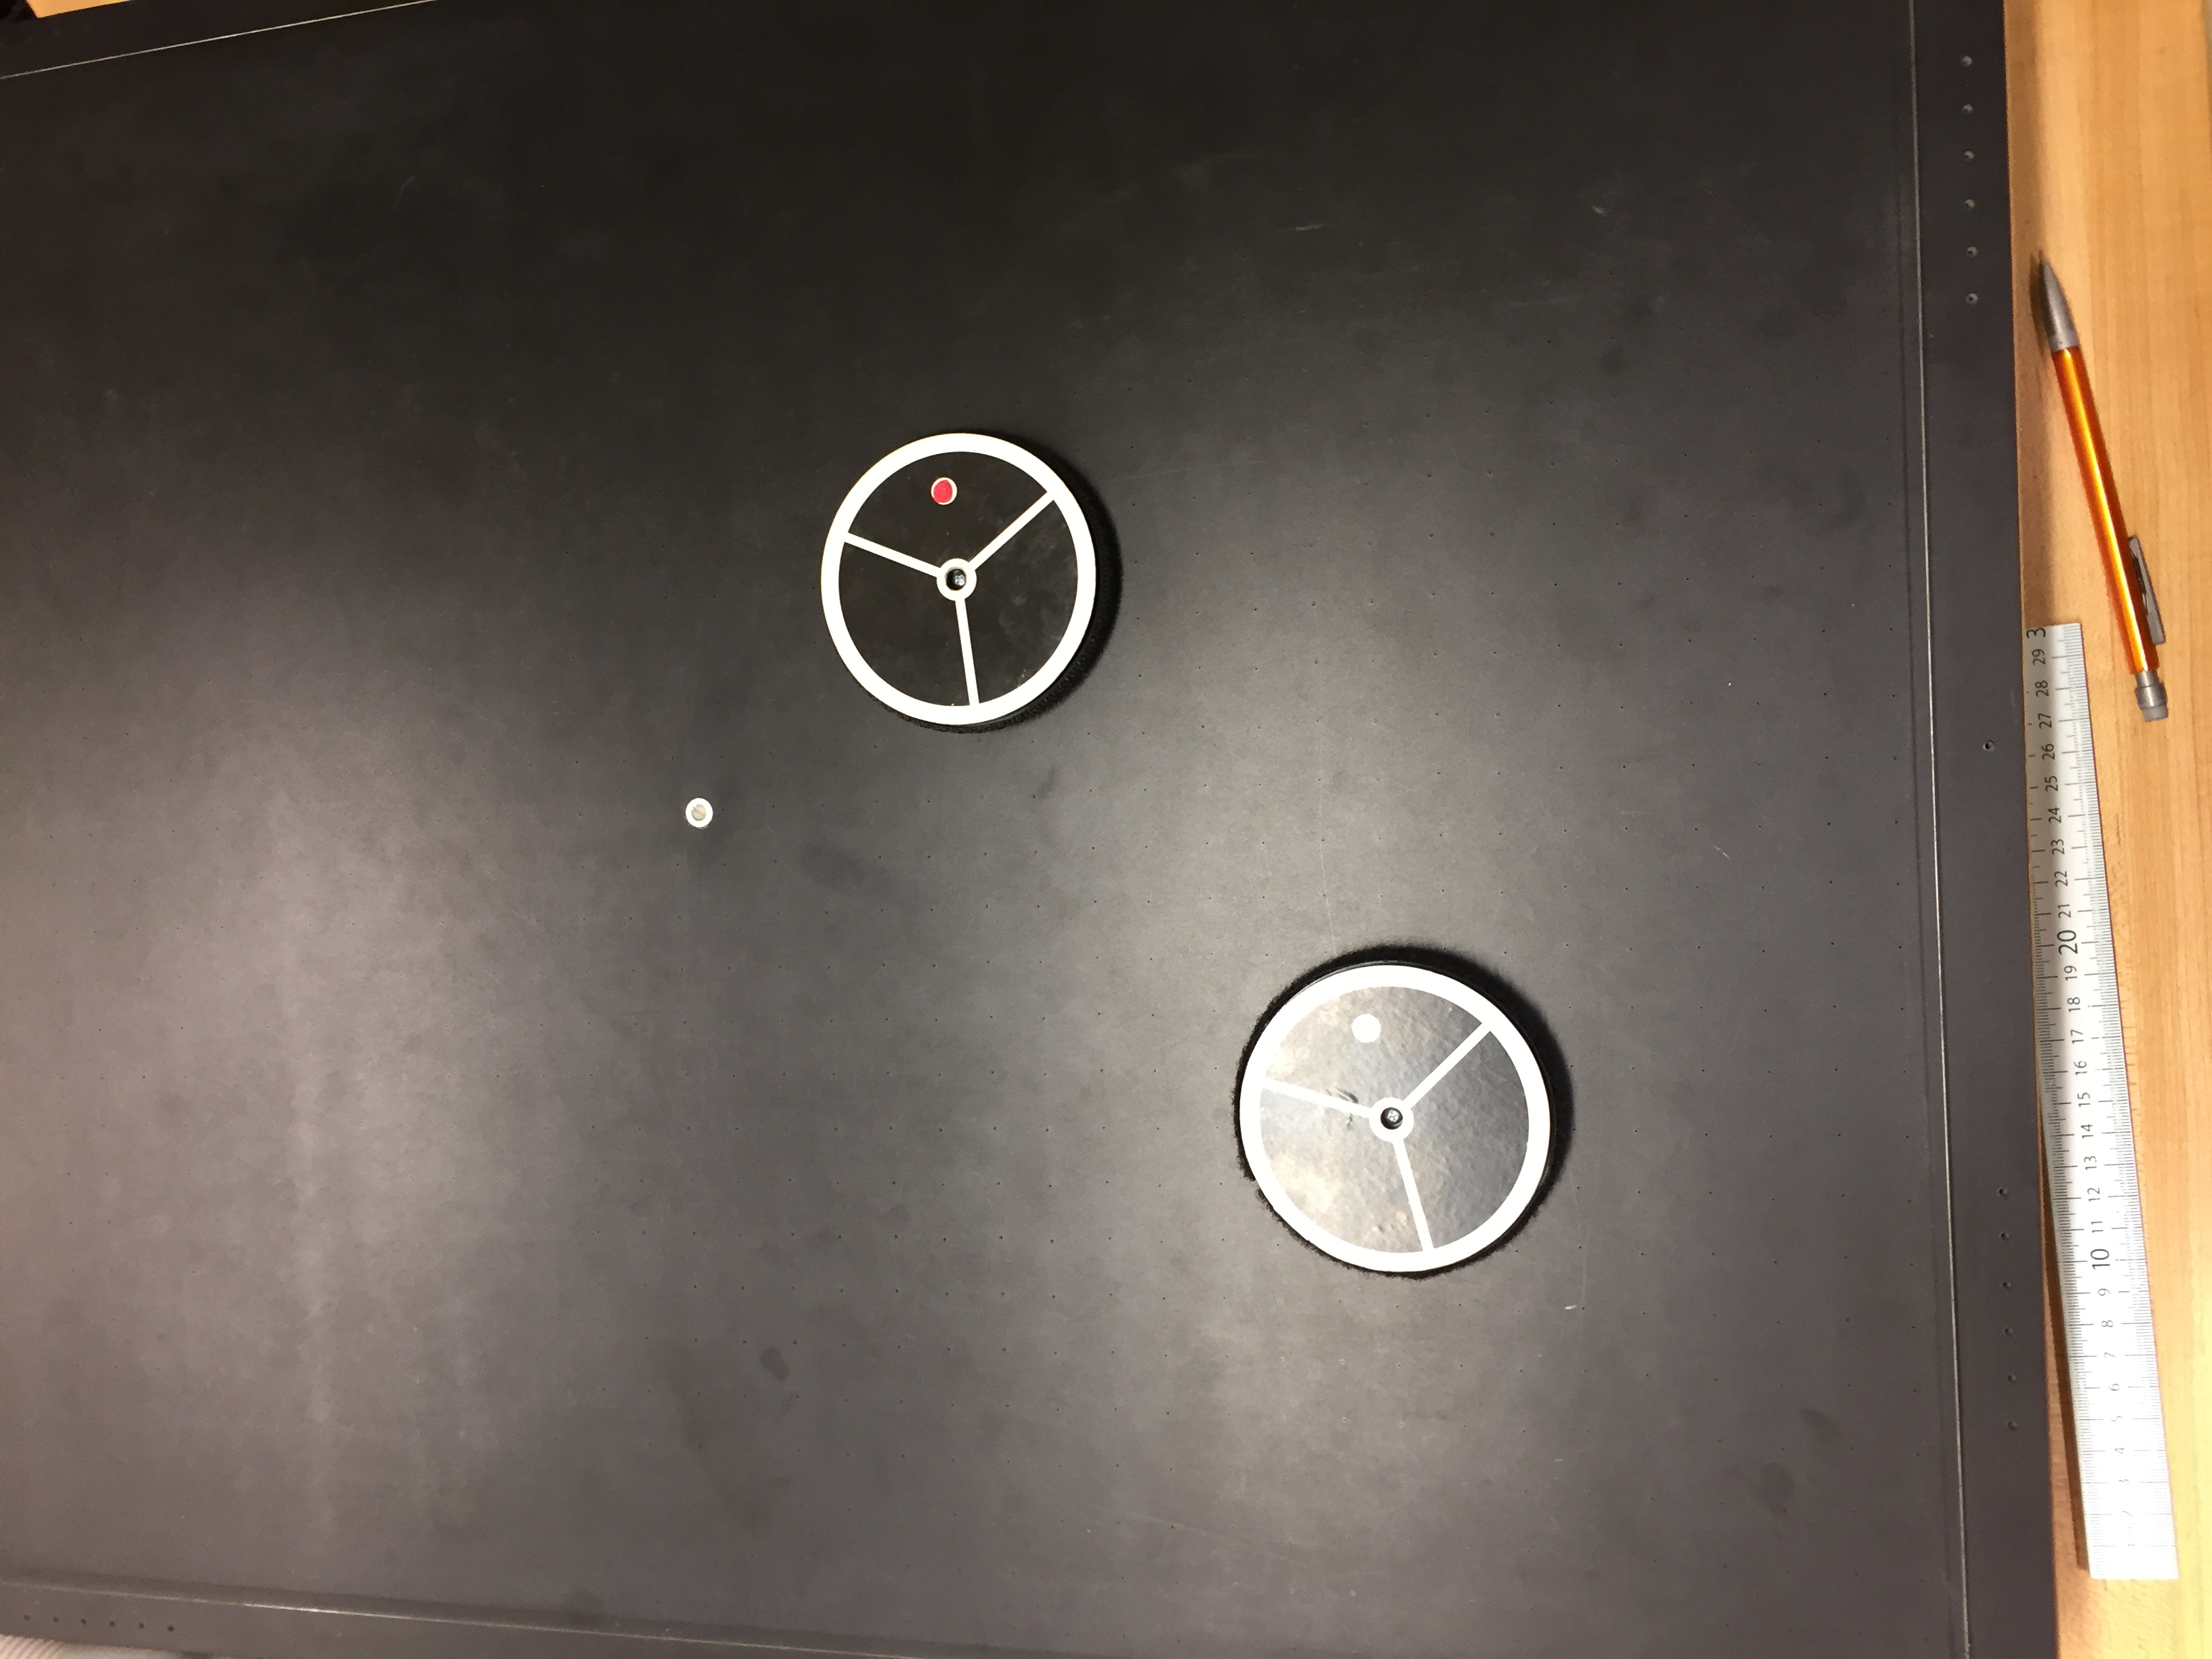
\includegraphics[scale = 0.06]{pucks.JPG}}{\caption{2 pucks on the airtable, along with a cm ruler on the right side.}\label{pucks}}
     \ffigbox{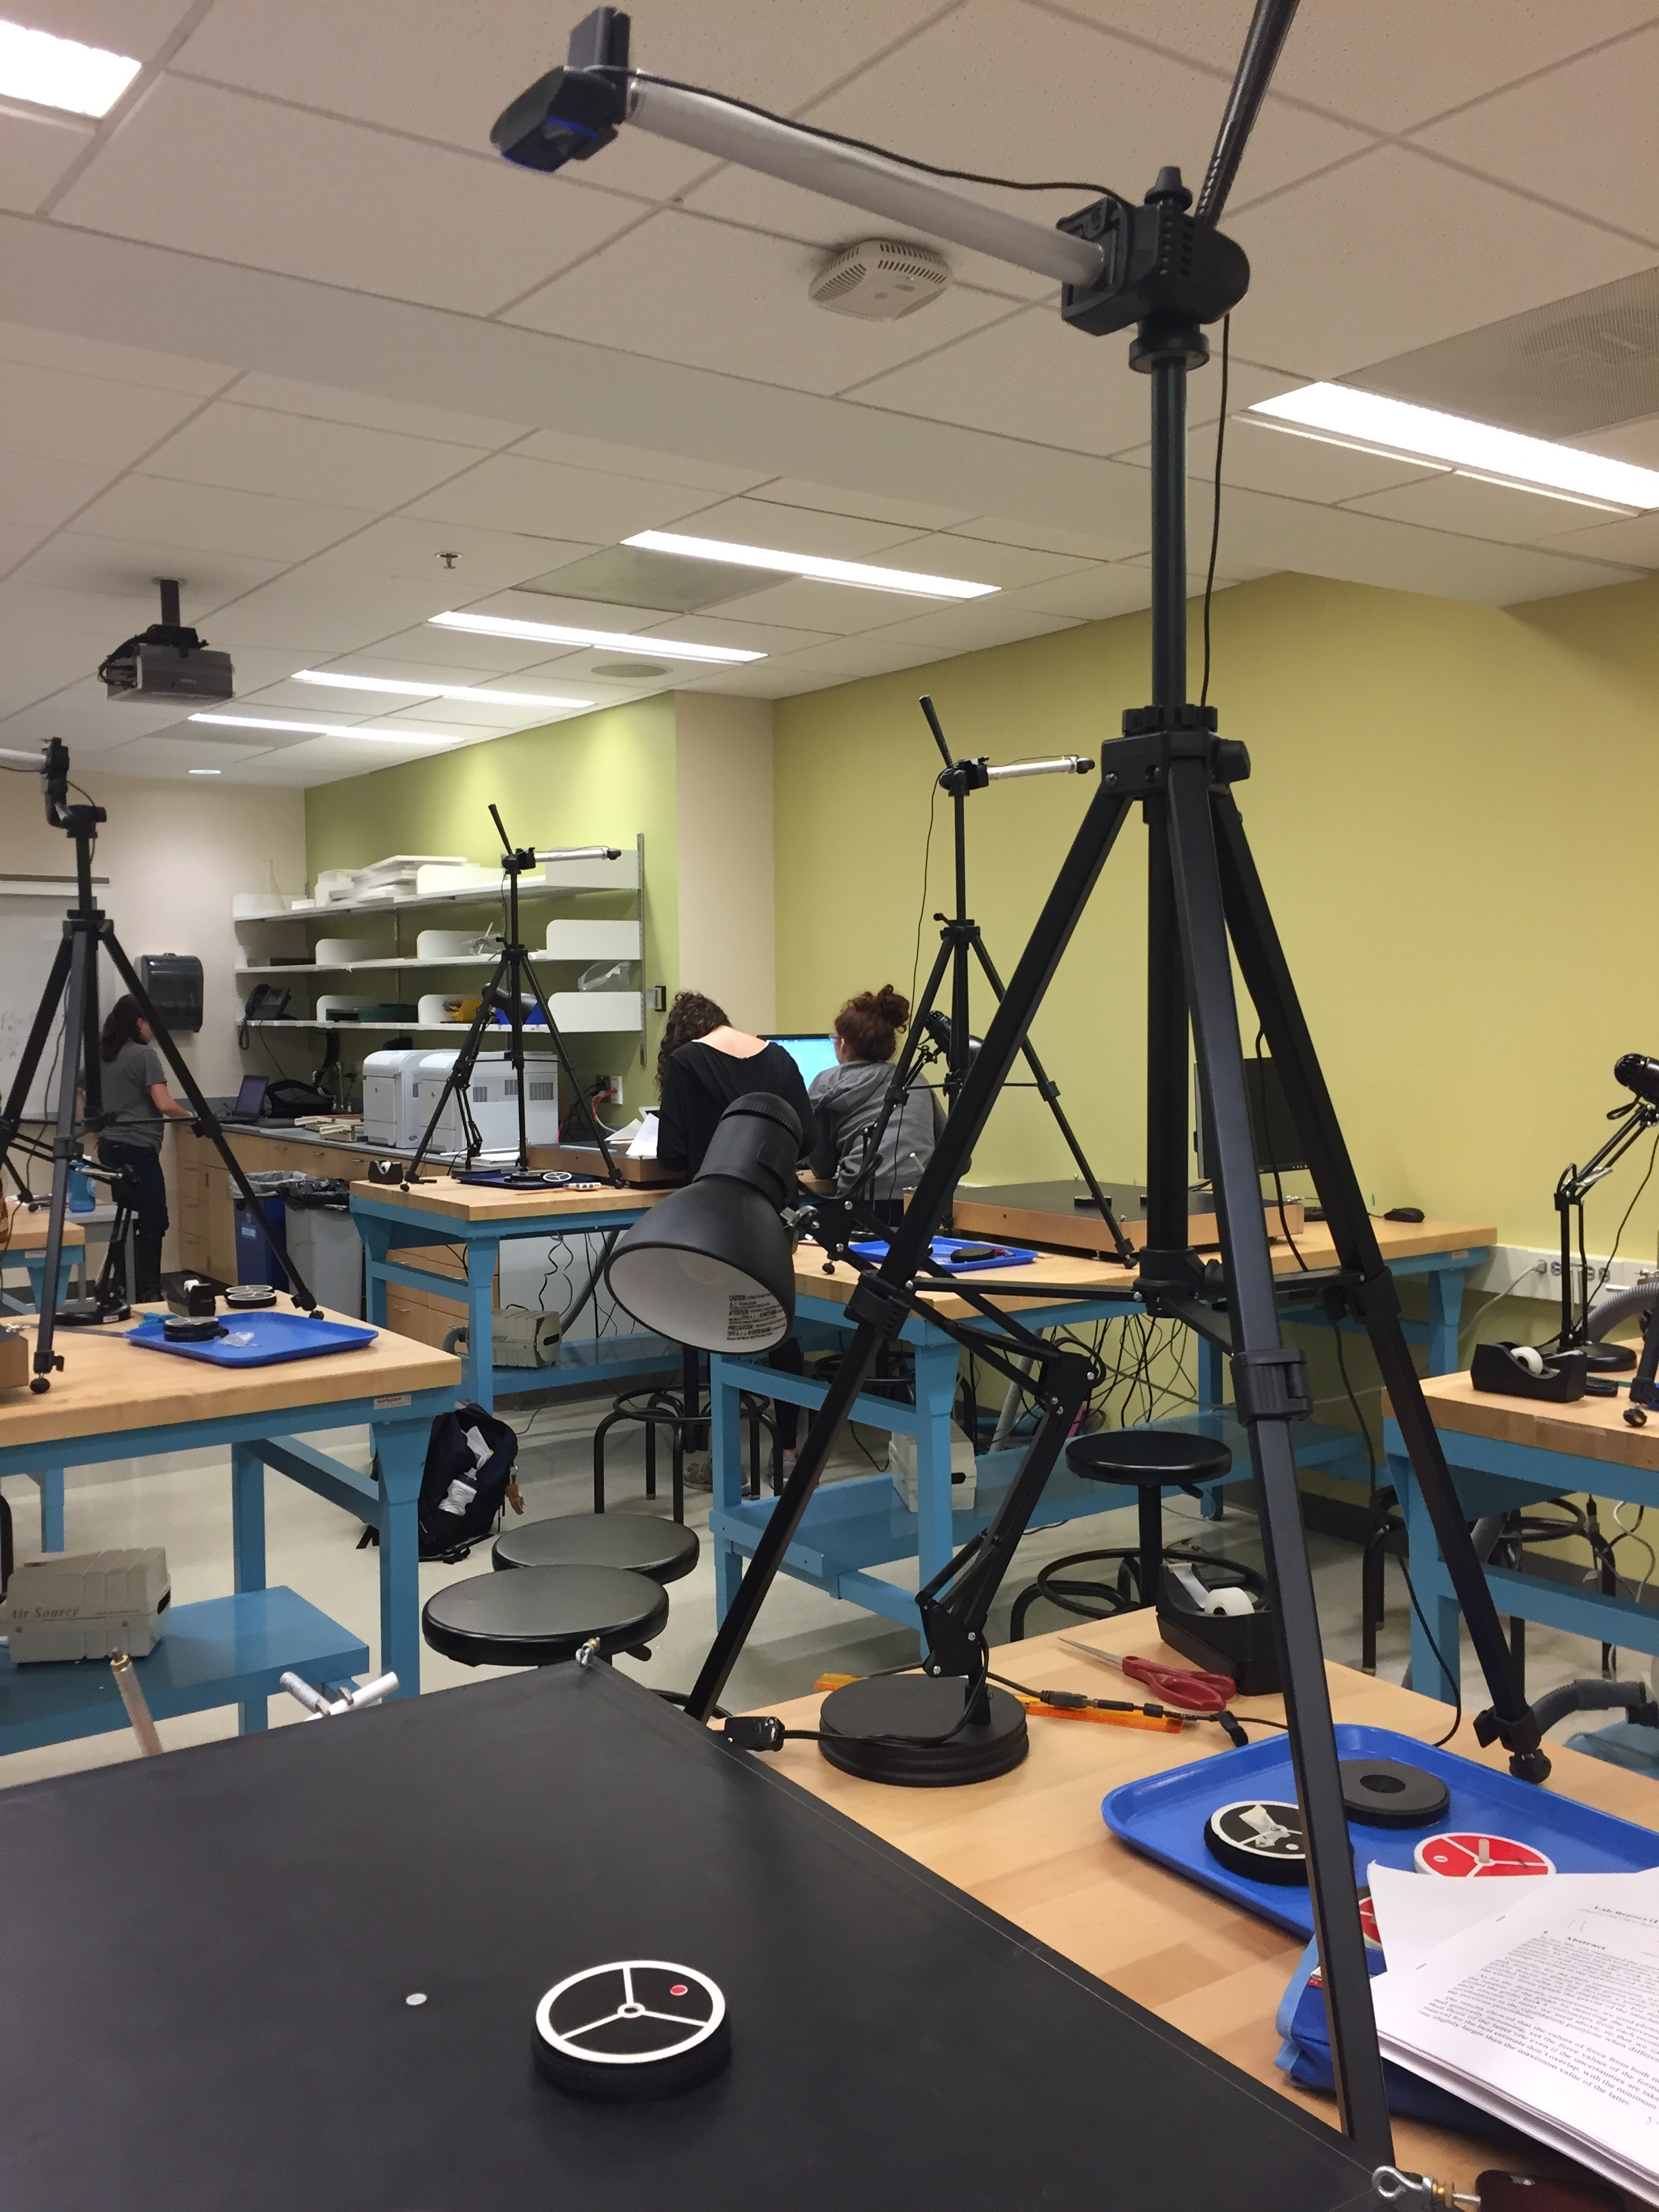
\includegraphics[scale = 0.06]{camera.JPG}}{\caption{View of camera suspended above pucks and table.}\label{cam}}
     % \ffigbox{\includegraphics[scale = 0.04]{airtank.JPG}}{\caption{A zoom}\label{zoom}}
   \end{floatrow}
\end{figure}

{\bf Experiment 1}\\

We weighed two magnetic pucks on the lab scale and made a mark on one to make sure we could distiguish one from the other. We then turned on the airtable and the camera and took a video of us throwing the pucks at each other, taking care to make sure that the throws had as little spin on them as possible. We then processed the video in Tracker as we have done in previous experiments, i.e. using the known length of the ruler as a marker to determine ground truth length in the camera images and manually marking the locations of the centers of the pucks. We then transferred our data from Tracker to Excel in order to process and analyze the data further.\\


{\bf Experiment 2}\\

We weighed two velcro-bound pucks on the lab scale and measured one of the radii with a cm ruler. As in the first experiment, we turned on the airtable and the camera and took a video of us throwing the pucks at each other, again attempting to throw with minimal spin. We then processed the video in Tracker in the same way as in the first experiment. After, we transferred our data from Tracker to Excel in order to process and analyze the data, as seen in the following section.




\section{Data Analysis}

{\bf Experiment 1}\\

Upon inspection of the data (see Figures \ref{xA}, \ref{xB}), I concluded that the interval of time prior to collision was from 0.000 seconds to 0.333 seconds (interval 1), the interval of time during the collision was between 0.333 seconds and 0.400 seconds (interval 2), and the post-collision interval was from 0.400 to 0.767 seconds (interval 3). Based on this breakdown of the time intervals, I used LINEST to calculate the slopes (velocities) and their associated standard deviations for each puck during intervals 1 and 3. Note that each uncertainty is the relevant standard deviation divided by square root of the number of measurements taken of the velocity, which in this case was only really one measurement since we only processed the video in Tracker once. My results were $v_{ix,A} = 0.744\pm0.011$ m/s, $v_{iy,A} = -0.302\pm0.005$ m/s, $v_{fx,A} = -0.738\pm0.011$ m/s, $v_{fy,A} = -0.289\pm0.006$ m/s, $v_{ix,B} = -0.644\pm0.038$ m/s, $v_{iy,B} = 0.261\pm0.015$ m/s, $v_{fx,B} = 0.556\pm0.004$ m/s, and $v_{fy,B} = 0.456\pm0.009$ m/s.

We would like to show that momentum and kinetic energy are conserved. To do so, we will first use the error propagation formula to properly calculate error on momentum and kinetic energy:

\begin{align}
\sigma_{P} = \sqrt{v^2\sigma_m^2+m^2\sigma_v^2}
\end{align}

and

\begin{align}
\sigma_{K} = \sqrt{\left(\frac{1}{2}v^2\right)^2\sigma_m^2+(mv)^2\sigma_v^2}
\end{align}

Assume that scale used to weigh the pucks has measurement precision of 0.001 kg, and so $\sigma_m=0.0005/\sqrt{1}=0.0005$ kg (we only weighed the pucks once each). Thus, we may calculate the values of initial and final momenta as seen in Table \ref{tabmom}, using the proper error propagation formula $P_{total} = P_A + P_B \pm \sqrt{\sigma_{P_A}^2+\sigma_{P_B}^2}$ for the respective initial and final values of $x$ and $y$ (see appendix for a sample calculation).

\begin{table}[]
\centering
\caption{Initial and final momenta in the x- and y-directions.}
\label{tabmom}
\begin{tabular}{|l|l|}
\hline
$P_{ix}$ & $0.00158\pm0.000891$ kg$\cdot$m/s   \\ \hline
$P_{iy}$ & $-0.000650\pm 0.000358$ kg$\cdot$m/s \\ \hline
$P_{fx}$ & $-0.00313\pm 0.000510$ kg$\cdot$m/s \\ \hline
$P_{fy}$ & $0.00325 \pm 0.000337$ kg$\cdot$m/s \\ \hline
\end{tabular}
\end{table}

% The propagation on the uncertainties of the errors is ...
Now, to find the measured value and uncertainty regarding the initial and final values, we calculate $\Delta P := P_{f}-P_{i} \pm \sqrt{\sigma_{P_{f}}^2+\sigma_{P_{i}}^2}$. So our measured values are $\Delta P_x = -0.00471 \pm 0.00103$ kg$\cdot$m/s and $\Delta P_y = 0.00390 \pm 0.000492$ kg$\cdot$m/s.

Since we expected to find $\Delta P = 0$ for both cases, we find that

\begin{align}
\ceil*{\left\vert\frac{\Delta P_{measured_x}-\Delta P_{expected_x}}{\sigma_{measured_x}}\right\vert} = \ceil*{\left\vert\frac{-0.00471}{0.00103}\right\vert} = 5
\label{errPx}
\end{align}

\begin{align}
\ceil*{\left\vert\frac{\Delta P_{measured_y}-\Delta P_{expected_y}}{\sigma_{measured_y}}\right\vert} = \ceil*{\left\vert\frac{0.00390}{0.00492}\right\vert} = 1
\label{errPy}
\end{align}
Thus, with regards to conservation of momentum, the measurements on $x$ were not within 1 standard deviation of the mean and therefore were not very accurate, but the measurements on $y$ were within 1 standard deviation and could be considered more accurate.

\begin{figure}[!h]
   \begin{floatrow}
     \ffigbox{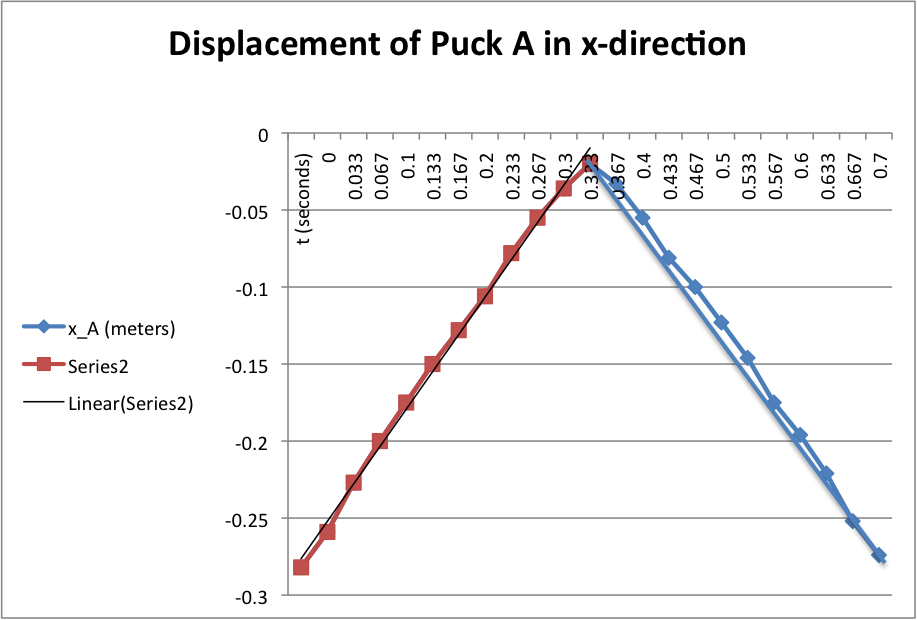
\includegraphics[scale = 0.5]{x_A.png}}{\caption{x-direction data points from Tracker for puck A with two lines of best fit.}\label{xA}}
     \ffigbox{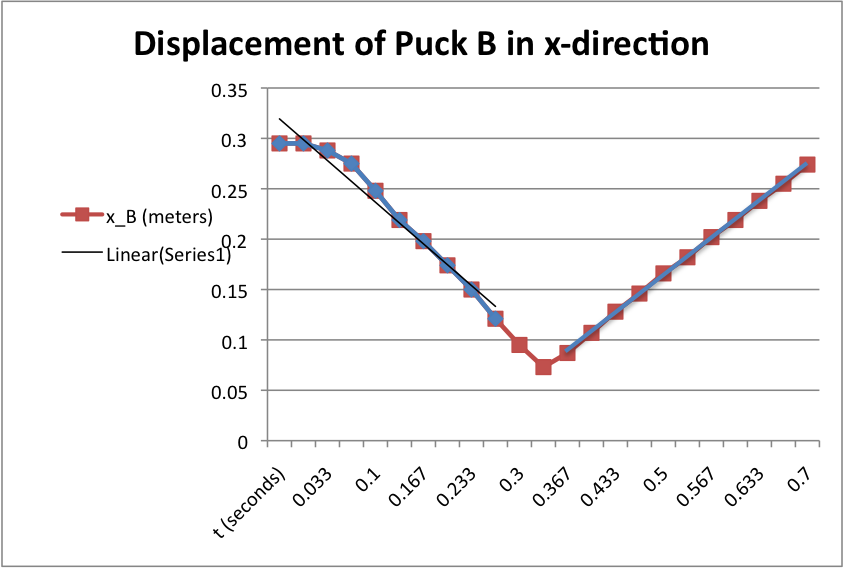
\includegraphics[scale = 0.54]{x_B.png}}{\caption{x-direction data points from Tracker for puck B with two lines of best fit.}\label{xB}}
     % \ffigbox{\includegraphics[scale = 0.04]{airtank.JPG}}{\caption{A zoom}\label{zoom}}
   \end{floatrow}
\end{figure}

\begin{figure}[!h]
   \begin{floatrow}
     \ffigbox{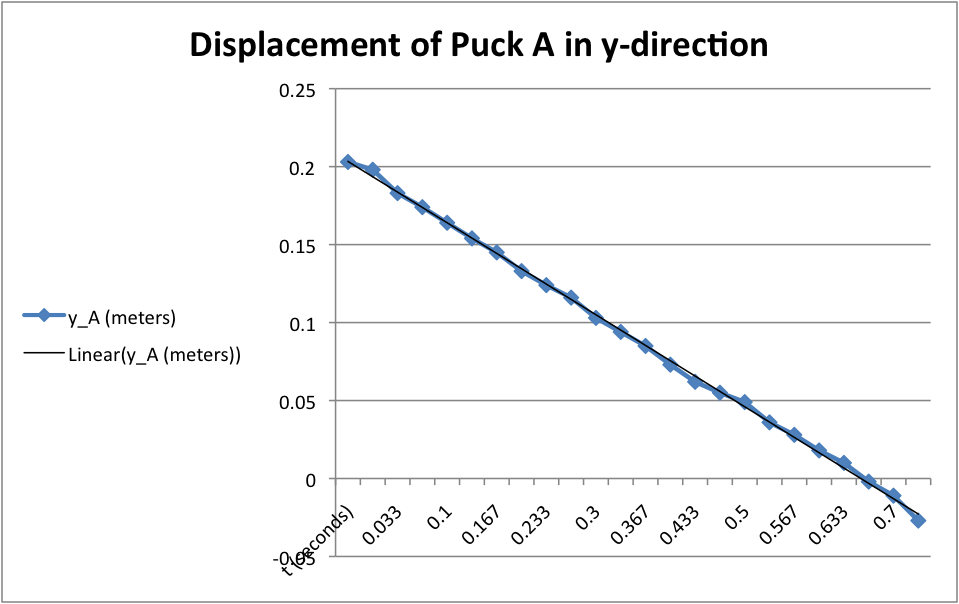
\includegraphics[scale = 0.48]{y_A.png}}{\caption{y-direction data points from Tracker for puck A with line of best fit.}\label{yA}}
     \ffigbox{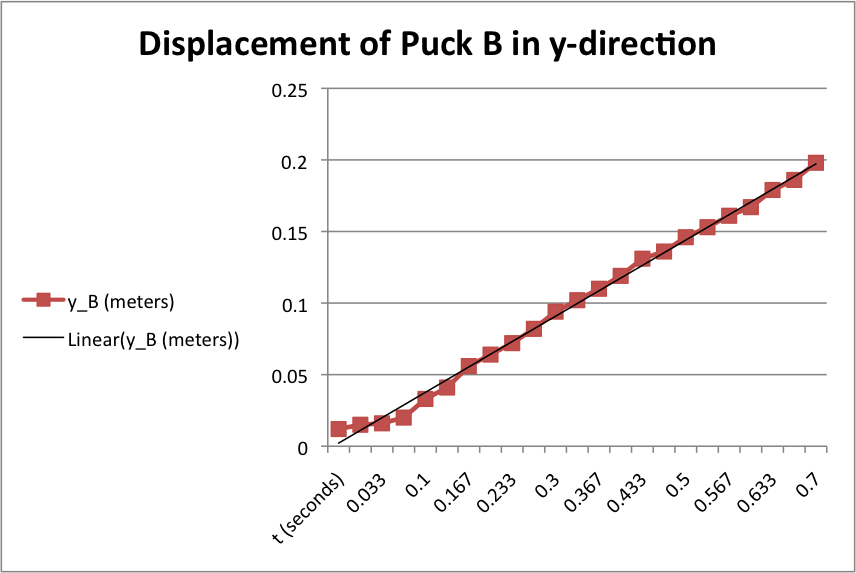
\includegraphics[scale = 0.51]{y_B.png}}{\caption{y-direction data points from Tracker for puck B with line of best fit.}\label{yB}}
     % \ffigbox{\includegraphics[scale = 0.04]{airtank.JPG}}{\caption{A zoom}\label{zoom}}
   \end{floatrow}
\end{figure}

We would also like to test whether our experiment shows conservation of kinetic energy, $K_f = K_i$. We calculate this by propagating error as $K_{total} = K_A+K_B \pm \sqrt{\sigma_{K_A}+\sigma_{K_B}}$ (see Appendix for sample calculation). The experimental values be seen in Table \ref{tabkin}.

\begin{table}[]
\centering
\caption{Initial and final kinetic energy in the x- and y-directions.}
\label{tabkin}
\begin{tabular}{|l|l|}
\hline
$K_{ix}$ & $0.00899\pm0.0000503$ J  \\ \hline
$K_{iy}$ & $0.00148\pm 0.0000819$ J \\ \hline
$K_{fx}$ & $0.00792\pm 0.0000206$  J \\ \hline
$K_{fy}$ & $0.00272 \pm 0.0000861$  J\\ \hline
\end{tabular}
\end{table}

Similarly to the calculation of momenta, we find the measured value and uncertainty by calculating $\Delta K := K_{f}-K_{i} \pm \sqrt{\sigma_{K_{f}}^2+\sigma_{K_{i}}^2}$. Our measured values are $\Delta K_x = -0.00107 \pm 0.0000543$ J and $\Delta K_y = 0.00124\pm 0.000119$ J.

Again, since we expected $\Delta K = 0$ J, we calculate

\begin{align}
\ceil*{\left\vert\frac{\Delta K_{measured_x}-\Delta K_{expected_x}}{\sigma_{measured_x}}\right\vert} = \ceil*{\left\vert\frac{-0.00107}{0.0000543}\right\vert} = 20
\label{errKx}
\end{align}

\begin{align}
\ceil*{\left\vert\frac{\Delta K_{measured_y}-\Delta K_{expected_y}}{\sigma_{measured_y}}\right\vert} = \ceil*{\left\vert\frac{0.00124}{0.000119}\right\vert} = 11
\label{errKy}
\end{align}


{\bf Experiment 2}\\

In this experiment, we used different pucks with velcro on them. Upon weighing, we found $m_A = 0.0016 \pm 0.0005$ kg, $m_B = 0.0017 \pm 0.0005$.

We took the raw displacement data from Tracker and transformed it into center of mass coordinates. For puck A, the formula we used was

\begin{align}
x_{A,cm}=x_A-\frac{m_A x_A+ m_B x_B}{m_A + m_B}
\end{align}

and we used an analogous formula for puck B. Analyzing the data (see Figures \ref{xA2}, \ref{xB2}), I identified the time interval prior to collision as from 0.000 seconds to 0.367 seconds. 

\begin{figure}[!h]
   \begin{floatrow}
     \ffigbox{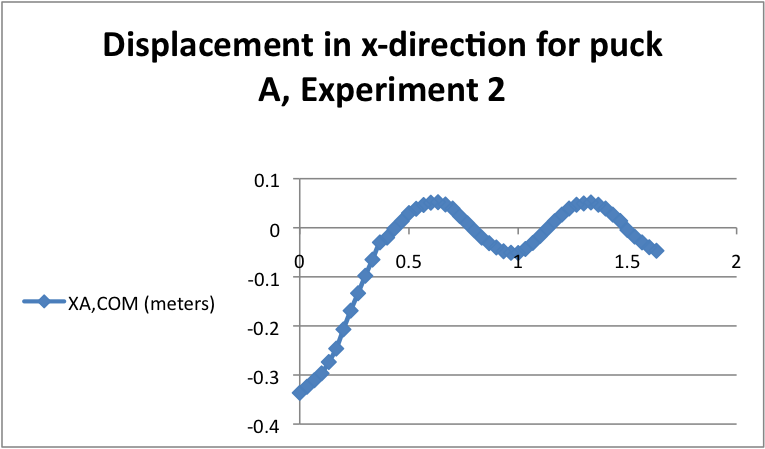
\includegraphics[scale = 0.58]{x_A2.png}}{\caption{x-direction data points from Tracker for puck A (position in meters vs time in seconds).}\label{xA2}}
     \ffigbox{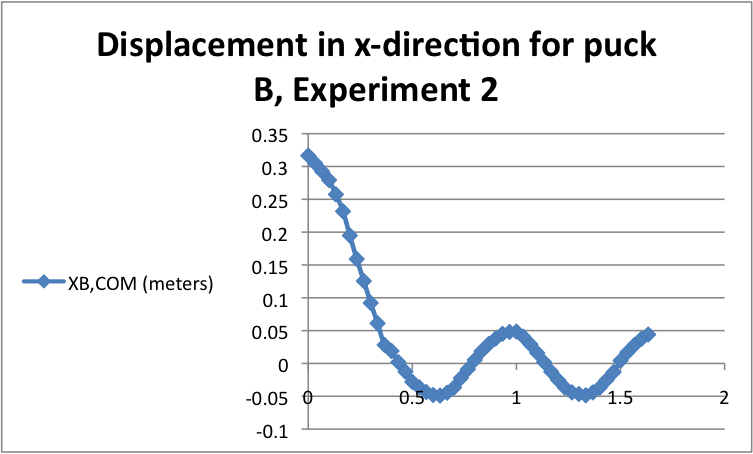
\includegraphics[scale = 0.57]{x_B2.png}}{\caption{x-direction data points from Tracker for puck B (position in meters vs time in seconds).}\label{xB2}}
     % \ffigbox{\includegraphics[scale = 0.04]{airtank.JPG}}{\caption{A zoom}\label{zoom}}
   \end{floatrow}
\end{figure}

\begin{figure}[h]
\centering
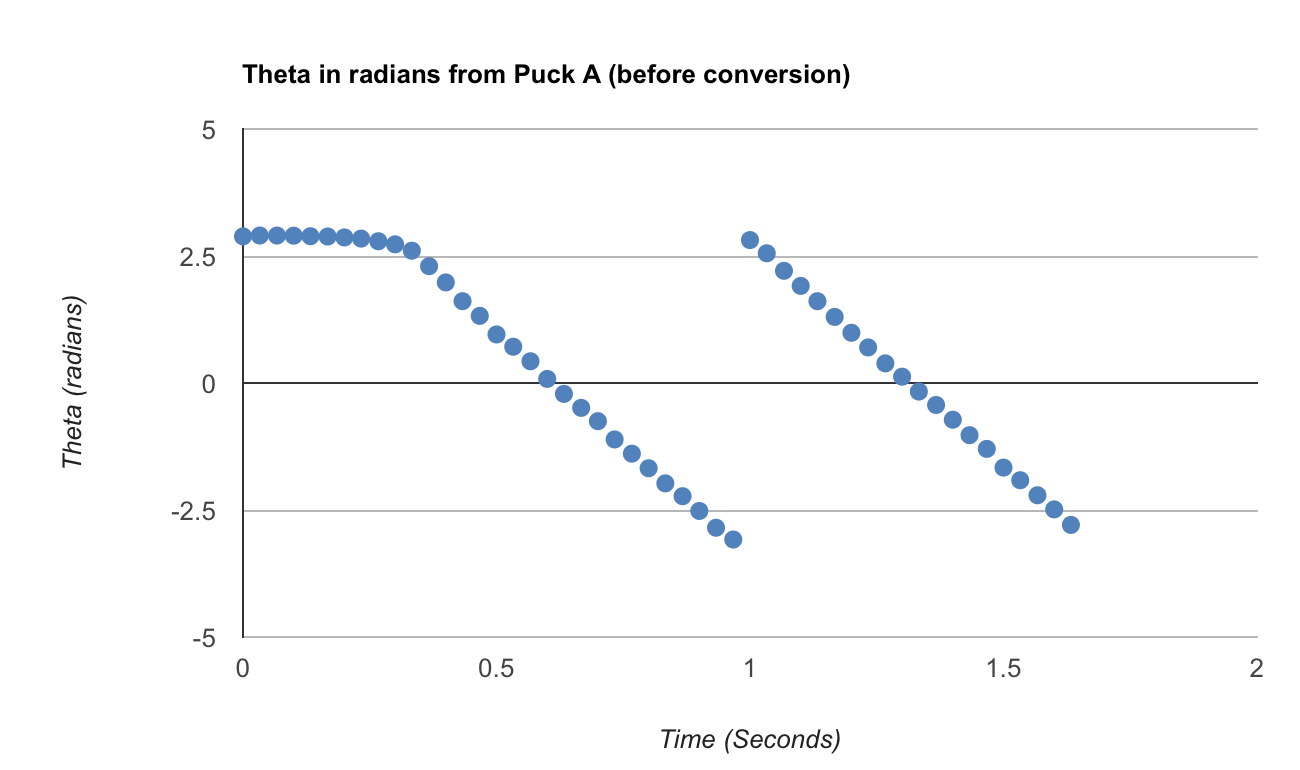
\includegraphics[width=.8\textwidth]{theta.png}
\caption{Angle data from Puck A.}
\label{theta}
\end{figure}

We used the ATAN2 function to calculate $\theta$ of each puck. As can be seen in Figure \ref{theta}, there is a discontinuity at $t=1$ seconds in the data for puck A. For the data for puck B, there is a similar discontinuity at $t=0.6$ seconds. At that point, we must subtract $2\pi$ from the data in order to alleviate the discontinuity. Taking the angle data from before and after $t=0.367$ seconds, we use LINEST to find $\omega_{A_i}=-1.161\pm0.295$ rad/s, $\omega_{A_f} = -8.937\pm0.0165$ rad/s, $\omega_{B_i}=-1.161\pm0.295$, and $\omega_{B_f} = -3.404\pm 0.793$ rad/s. These are all angular velocities; initial angular momentum can be found from finding the moment of inertia for each puck and multiplying it with their respective initial angular velocities:

\begin{align}
L_i &= \omega_{A_i}I_A + \omega_{B_i}I_B\\
&=  \omega_{A_i}m_1 r_1^2 + \omega_{B_i}m_2 r_2^2
\end{align}

where $r$ is the norm of $x_{cm}, y_{cm}$. The error propagation on $I\omega $ is $\sigma_{I\omega} = \sqrt{\omega^2\sigma_I^2 + I^2\sigma_{\omega}^2}$ and on $L_i$ it is $\sigma_{L_i} = \sqrt{\sigma_{L_{iA}}^2+\sigma_{L_{iB}}^2}$. In this case, this leads to $L_i = 0.000374\pm 0.000824$ kg $m^2/s$. In the final calculation of angular momentum, we use $I_f=\frac{3}{2}M_TR^2$, where $R$ is the radius of one of the pucks. Thus we have

\begin{align}
L_f = I_f(\omega_{A_f}+ \omega_{B_f})
\end{align}

Error propagation on $I_f$ is $\sigma_{I_f} = \sqrt{\frac{9}{4}R^4\sigma_{M_T}^2+9M_T^2R^2\sigma_{R}^2}$. Error propagation on $L_f$ is $\sqrt{\sigma_{L_{fA}}+\sigma_{L_{fA}}}$. Assuming uncertainty in radial measurement of $\pm 0.0005$ meters, we find $L_f = -0.000135\pm 0.000628$ kg $m^2$/s. So using methods of calculation of error propagation similar to the previous ones, $\Delta L = -0.000509 \pm 0.00104$. Since we expected $\Delta L = 0$ by conservation of angular momentum, we calculate:

\begin{align}
\ceil*{\left\vert\frac{\Delta L_{measured}-\Delta L_{expected}}{\sigma_{\Delta L}}\right\vert} = \ceil*{\left\vert\frac{-0.000509}{0.00104}\right\vert} = 1
\label{errL}
\end{align}

We would also like to test our hypothesis regarding conservation of linear momentum, but in this case the system seems to experience perturbations soon after the collision (see Figures \ref{xA2}, \ref{xB2}), and so there is very little data for the final linear momentum. We do so similarly to experiment 1, using the interval from 0.000 seconds to 0.367 seconds as the initial interval and 0.400 to 0.633 seconds as the second interval and find $v_{ix,A} = 0.879\pm0.0453$ m/s, $v_{iy,A} = -0.144\pm0.00435$ m/s, $v_{fx,A} = 0.314\pm0.0365$ m/s, $v_{fy,A} = -0.267\pm0.0450$ m/s, $v_{ix,B} = -0.825\pm0.0427$ m/s, $v_{iy,B} = 0.135\pm0.00410$ m/s, $v_{fx,B} = -0.295\pm0.0344$ m/s, and $v_{fy,B} = 0.251\pm0.0424$ m/s. Using the same error propagation as in experiment 1, we find initial and final momenta, shown in Table \ref{mom2}. From these values, and via error propagation, we find $\Delta P_x = -3.00\times10^{-6}\pm1.70\times 10^{-4}$ kg$\cdot(m/s)$ and $\Delta P_y = 4.00\times10^{-7}\pm2.50\times10^{-4}$ kg$\cdot(m/s)$.

\begin{table}[]
\centering
\caption{Initial and final momenta in experiment 2.}
\label{mom2}
\begin{tabular}{|l|l|}
\hline
$P_ix$ & $3.90\times10^{-6}\pm6.70\times10^{-7}$ kg$\cdot(m/s)$   \\ \hline
$P_iy$ & $-9.00\times10^{-7}\pm 7.30\times10^{-8}$ kg$\cdot(m/s)$ \\ \hline
$P_fx$ & $9.00\times10^{-7}\pm 3.00\times 10^{-8}$  kg$\cdot(m/s)$ \\ \hline
$P_fy$ & $-5.00\times10^{-7} \pm 6.00\times 10^{-8}$ kg$\cdot(m/s)$\\ \hline
\end{tabular}
\end{table}

We again expected linear momentum to be conserved and so calculate

\begin{align}
\ceil*{\left\vert\frac{\Delta P_{measured_x}-\Delta P_{expected_x}}{\sigma_{measured_x}}\right\vert} = \ceil*{\left\vert\frac{-3.00\times10^{-6}}{1.70\times 10^{-4}}\right\vert} = 1
\label{errPx2}
\end{align}

\begin{align}
\ceil*{\left\vert\frac{\Delta P_{measured_y}-\Delta P_{expected_y}}{\sigma_{measured_y}}\right\vert} = \ceil*{\left\vert\frac{4.00\times10^{-7}}{2.50\times10^{-4}}\right\vert} = 1
\label{errPy2}
\end{align}
With such low error, our values allow us to reasonably conclude that linear momentum was conserved in experiment 2.

As for kinetic energy, we do not expect it to be conserved in this case, since we have an inelastic collision. We have total initial kinetic energy of the system given by 

\begin{align}
K_i = \frac{1}{2}(m_A v_{A,i}^2 + I_A \omega_{A,i}^2 + m_B v_{B,i}^2 +I_B \omega_{B,i}^2)
\end{align}

After the collision, the equation for kinetic energy simplifies to 

\begin{align}
K_f =\frac{1}{2}I(\omega_A^2+\omega_B^2)
\end{align}

Error propagation for $K_i$ gives $\sigma_{K_i} = \frac{1}{2}\sqrt{\sigma_{K_{A,i}}^2+\sigma_{K_{B,i}}^2}$, with $\sigma_K = \sqrt{\sigma_{K_{linear}}^2+\sigma_{K_{angular}}^2}$, for $K_{A,i}=\frac{1}{2}(m_A v_{A,i}^2+I_A \omega_{A,i}^2)$ and analogously for $K_{B,i}$, and so $\sigma_{K_{linear}}=\sqrt{(1/2v^2)^2\sigma_m^2+(mv)^2\sigma_v^2}$ and $\sigma_{K_{angular}}=\sqrt{(1/2\omega^2)^2\sigma_I^2+(I\omega)^2\sigma_{\omega}^2}$. Error propagation for $K_f$ gives $\sigma_{K_f}=\frac{1}{2}\sqrt{\sigma_{K_{A,f}}^2+\sigma_{K_{B,f}}^2}$, and in this case each term only has a contribution from angular momentum.

With these considerations taken into account, we may finally calculate initial and final kinetic energy for the system: $K_i = 1.19\times10^{-3} \pm3.00\times10^{-5}$ J and $K_f = 1.00\times10^{-3} \pm7.00\times10^{-5}$ J. 


\section{Conclusions}

I calculated many values in this lab: for experiment 1, I found initial and final linear momenta, as seen in Table \ref{tabmom}, and initial and final kinetic energies, as seen in Table \ref{tabkin}; for experiment 2, I found initial and final linear momenta, as seen in Table \ref{mom2}, final angular momenta, $L_f = -0.000135\pm 0.000628$ kg $m^2$/s (assuming $L_i=0$ kg $m^2$/s for a straight throw of the pucks), and initial and final kinetic energies, $K_i = 1.19\times10^{-3} \pm3.00\times10^{-5}$ J and $K_f = 1.00\times10^{-3} \pm7.00\times10^{-5}$ J. 


We conclude within reasonable statistical error that momentum was conserved in both experiments (see equations \ref{errPx}, \ref{errPy}, \ref{errPx2}, \ref{errPy}), but that kinetic energy was only conserved in the first experiment, which was an elastic collision.

A source of experimental error may have been that my or my partner's hand interacted with the pucks for longer than we meant when we threw the pucks across the board and so the model of interactions may not have been accurate, since they were not formulated to account for hand interaction with the puck. Also, our calculations took place in the x-y plane, while the real experiment took place in 3-space, and therefore the measurements of displacement may have been distorted by our assumption that the camera and table were exactly parallel to one another.



% \begin{figure}[!h]
%    \begin{floatrow}
%      \ffigbox{\includegraphics[scale = 0.4]{histdown.png}}{\caption{Frequency of downward acceleration values.}\label{histdown}}
%      \ffigbox{\includegraphics[scale = 0.4]{histup.png}}{\caption{Frequency of upward acceleration values.}\label{histup}}
%      % \ffigbox{\includegraphics[scale = 0.04]{airtank.JPG}}{\caption{A zoom}\label{zoom}}
%    \end{floatrow}
% \end{figure}

\section{Appendix}
Example calculation of initial momentum from Experiment 1:\\
\begin{align*}
P_{ix} =& m_A v_{ix,A} + m_B v_{ix,B} \pm \sqrt{\sigma_{P_{ix,A}}^2+\sigma_{P_{ix,B}}^2} \\
=& 0.0184\cdot0.744 + 0.0188\cdot(-0.644) \\
&\pm \sqrt{0.744^2\cdot0.0005^2+0.0184^2\cdot0.011^2+0.644^2\cdot0.0005^2+0.0188^2\cdot0.038^2} \\
=& 0.00158\pm0.000891 kg\cdot m/s
\end{align*}

Example calculation of initial kinetic energy from Experiment 1:\\
\begin{align*}
K_{ix} =& \frac{1}{2}m_A v_{ix,A}^2 + m_B v_{ix,B}^2 \pm \sqrt{\sigma_{K_{ix,A}}^2+\sigma_{K_{ix,B}}^2} \\
=& \frac{1}{2}0.0184\cdot0.744^2 + \frac{1}{2}0.0188\cdot(-0.644)^2 \\
&\pm \sqrt{(\frac{1}{2}0.744^2)^2\cdot0.0005^2+(0.0184\cdot0.744)^2\cdot0.011^2+(\frac{1}{2}0.644^2)^2\cdot0.0005^2+(0.0188\cdot0.644)^2\cdot0.038^2} \\
=& 0.00899\pm0.0000503 J
\end{align*}
% Example velocity calculation:
% \begin{align}
% y'(0.0814) = \frac{y(0.111) - y(0.0814)}{0.111-0.0814}
% \end{align}


\begin{figure}[h]
\centering
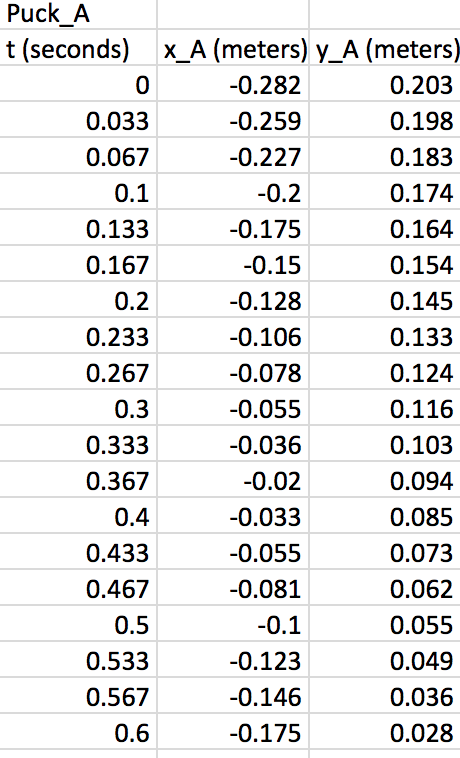
\includegraphics[width=.4\textwidth]{exp1.png}
\caption{Partial set of raw displacement data from experiment 1.}
\end{figure}

\begin{figure}[h]
\centering
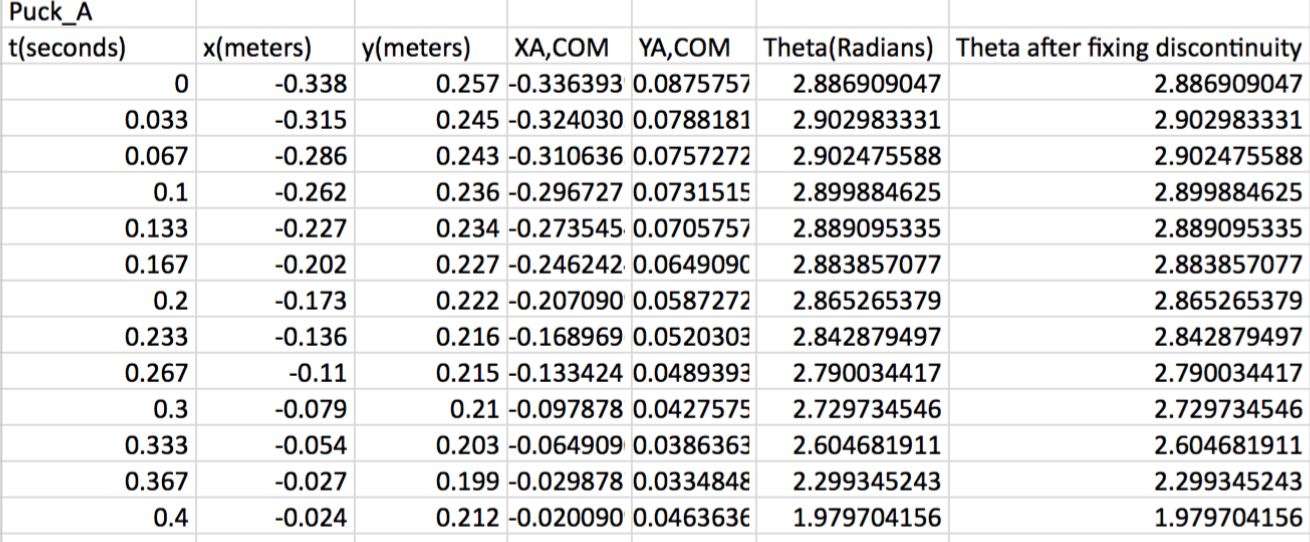
\includegraphics[width=.8\textwidth]{exp2.png}
\caption{Partial set of raw displacement and transformed data from experiment 2.}
\end{figure}

% \begin{figure}[h]
% \centering
% \includegraphics[width=.6\textwidth]{dyndata.png}
% \caption{Example of raw data from photogate.}
% \end{figure}

% \begin{figure}[h]
% \centering
% \includegraphics[width=.4\textwidth]{numint.png}
% \caption{Using static force data to calculate numerical integral of work.}
% \end{figure}

% Shareable link to all data and calculations in Google Sheets:\\
% \url{https://docs.google.com/spreadsheets/d/1iPam2b1wJpN4SLBrfSpwEydir6UGfoj3ltHsdv_Kwsw/edit?usp=sharing}

% \begin{figure}[h]
% \centering
% \includegraphics[width=.4\textwidth]{exdata.png}
% \caption{Example of raw data from processing video in Tracker.}
% \end{figure}



\end{document}
